\section{Auswertung}
\label{sec:Auswertung}

Im folgenden Kapitel wird die Justierung und Kalibrierung ausgewertet, sowie die
Lebensdauer des Myons anhand der Messdaten ermittelt. Die dabei auftretenden Fehlerrechnungen
werden mit dem \textit{uncertainties}-Paket in \textit{Python 3.6.6} berechnet. Für den Fehler der gemessenen $N$ wird
$\sqrt{N}$ angenommen, da diese poissonverteilt sein sollten.

\noindent
Zuerst wird die Justierung der Diskriminatoren ausgewertet, anschließend die
Kalibrierung des Vielkanalanalysators ausgewertet, und zum Schluß die Lebensdauer
ermittelt.

\subsection{Justierung der Diskriminatoren}
\label{sec:Verzögerungszeit}

Die gemessenen Signale $N(T_{\symup{VZ}})$ pro 10 Sekunden zu den jeweiligen Verzögerungszeiten sind in
Tabelle \ref{tab:verzoegerung} aufgelistet. Zusätzlich sind die Daten in Abbildung \ref{fig:verzoegerung}
dargestellt.

\begin{figure}[h]
  \centering
  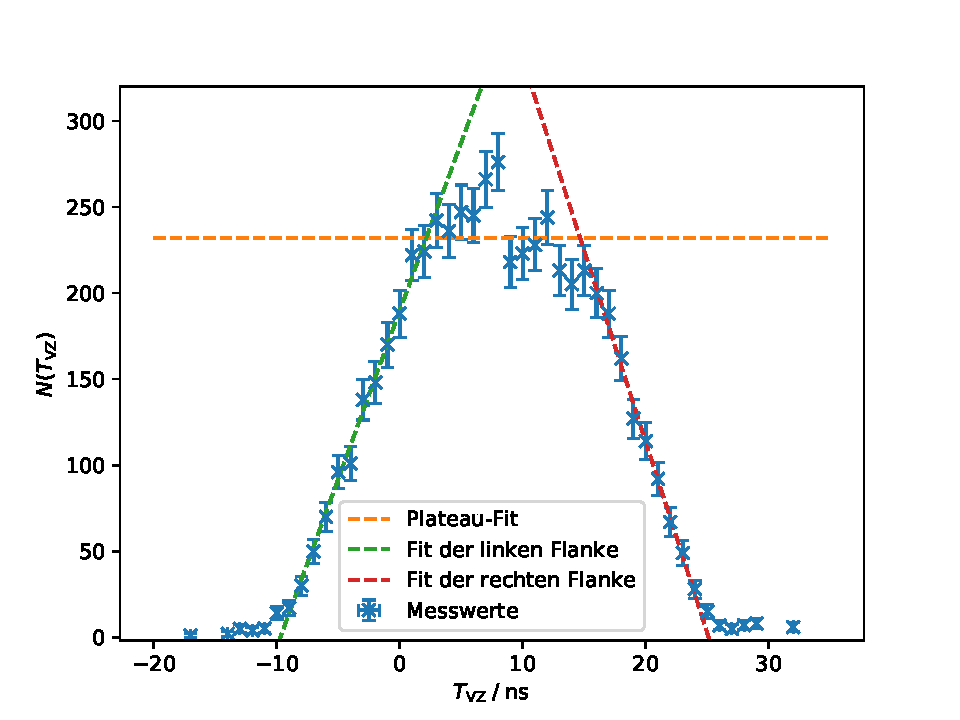
\includegraphics{verzoegerungregression.pdf}
  \caption{Die Gemessenen Signale $N(T_{\symup{VZ}})$ über der Verzögerungszeit $T_{\symup{VZ}}$. Dazu die Regressionsgeraden für die jeweiligen Bereiche.}
  \label{fig:verzoegerung}
\end{figure}

\begin{table}
  \centering
  \caption{Gemessene Signale zu eingestellten Verzögerungszeiten.}
  \label{tab:verzoegerung}
  \begin{tabular}{c c | c c | c c}
    \toprule
    $T_{\symup{VZ}}\;/\;\symup{ns}$ & $N(T_{\symup{VZ}})\;/\;\symup{s}^{-1}$ &
    $T_{\symup{VZ}}\;/\;\symup{ns}$ & $N(T_{\symup{VZ}})\;/\;\symup{s}^{-1}$ & $T_{\symup{VZ}}\;/\;\symup{ns}$ & $N(T_{\symup{VZ}})\;/\;\symup{s}^{-1}$\\
    \midrule
    -17 &  1  & 1  & 222  & 17 & 188 \\
    -14 &  2  & 2  & 224  & 18 & 162 \\
    -13 &  5  & 3  & 242  & 19 & 127 \\
    -12 &  4  & 4  & 236  & 20 & 114 \\
    -11 &  5  & 5  & 247  & 21 & 92  \\
    -10 &  14 & 6  & 245  & 22 & 67  \\
    -9  & 17  & 7  & 266  & 23 & 49  \\
    -8  & 30  & 8  & 276  & 24 & 28  \\
    -7  & 50  & 9  & 218  & 25 & 15  \\
    -6  & 70  & 10 &  223 & 26 & 7   \\
    -5  & 96  & 11 &  228 & 27 & 5   \\
    -4  & 101 & 12 &  244 & 28 & 7   \\
    -3  & 138 & 13 &  213 & 29 & 8   \\
    -2  & 148 & 14 &  205 & 32 & 6   \\
    -1  & 170 & 15 &  213            \\
     0  & 188 & 16 &  200            \\
    \bottomrule
  \end{tabular}
\end{table}

Durch das Plateau an Maximalwerten in Abbildung \ref{fig:verzoegerung} wird eine
Regressionsgerade mit Steigung 0 gelegt, um mittels Formel \ref{eqn:nmax} die
Maximalanzahl an Signalen pro 10 Sekunden zu erhalten.
\begin{equation}
  N(T_{\symup{VZ}}) = 0\,\cdot\,T_{\symup{VZ}}\;+\;N_{\symup{max}}
  \label{eqn:nmax}
\end{equation}
Es ergibt sich ein $N_{\symup{max}} = 232 \pm 4$.

\noindent
Als nächstes wird mithilfe des
Maximalwerts die Halbwertsbreite, und damit die Breite des Plateaus, bestimmt.
Dafür werden zunächst Regressionsgeraden durch die Flanken gelegt, um die Verzögerungszeiten
zu erhalten, bei denen die Signalanzahl auf $N_{\symup{max}}/2$ gesunken ist.
\begin{equation}
  N(T_{\symup{VZ}}) = \symup{a}\,\cdot\,T_{\symup{VZ}}\;+\;\symup{b}
  \label{eqn:flanke}
\end{equation}
Nach \ref{eqn:flanke} ergeben sich folgende a und b für die linke bzw. rechte Flanke:
\begin{align*}
  \text{Linke Flanke:\;}\\
  \symup{a_l} &= (19,5\;\pm\;0,8)\,\frac{1}{\symup{ns}}\\
  \symup{b_l} &= 190\;\pm\;6\\
  \text{Rechte Flanke:\;}\\
  \symup{a_r} &= (-22,2\;\pm\;1,6)\,\frac{1}{\symup{ns}}\\
  \symup{b_r} &= 557\;\pm\;33\\
\end{align*}
Setzt man $N(T_{\symup{VZ}})$ gleich $N_{\symup{max}}/2$, ergeben sich:
\begin{align*}
  T_{\symup{VZ,L}} &= (-3,8\;\pm\;0,4)\,\symup{ns}\\
  T_{\symup{VZ,R}} &= (19,9\;\pm\;2,1)\,\symup{ns}\\
\end{align*}
Damit ergibt sich eine Breite des Plateaus von
\begin{equation*}
  T_{\symup{VZ,Gesamt}} = T_{\symup{VZ,L}}\;+\;T_{\symup{VZ,R}} = (23,7\;\pm\;2,1)\,\symup{ns}.
\end{equation*}
Da sich die Breite gerade aus den Plateaubreiten der Rechtecksignale der beiden SEV
ergibt, wird eine Breite knapp über $\SI{24}{\nano\second}$ erwartet. %8ns

Es wird eine Verzögerungszeit ($\SI{8}{\nano\second}$) innerhalb des Plateaus eingestellt, um eine
maximale Zählrate der Koinzidenzapparatur zu erreichen.

\subsection{Kalibrierung des Vielkanalanalysators}
\label{sec:vielkanalanalysator}

Die Kalibrierung des Vielkanalanalysators wird verwendet, um eine Umrechnung der
Channels $c$ des Analysators auf Zeitabstände $t$ zu ermöglichen.
\begin{equation}
  t(c) = \symup{a}\,\cdot\,c\;+\;\symup{b}
  \label{eqn:zeit}
\end{equation}
Dafür werden mittels Formel \ref{eqn:zeit}
die vom Doppelimpulsgenerator gefüllten Channels in Verbindung mit den eingestellten
Zeitabständen gebracht. Mit einer Regressionsgeraden durch die in Tabelle \ref{tab:zeit} aufgelisteten Messwerte werden a und b bestimmt:
\begin{align*}
  \symup{a} &= (0,022348\;\pm\;0,000012)\,\symup{\mu s}\\
  \symup{b} &= (-0,033\;\pm\;0,003)\,\symup{\mu s}\\
\end{align*}
%Dabei werden die in Tabelle \ref{tab:zeit} mit einem Sternchen markierten Werte in der Regression
%nicht beachtet, da in dem Fall der Doppelimpulsgenerator für eine Zeit zwei Channels füllte.
%Dabei handelt es sich in Tabelle \ref{tab:zeit} um die mit Sternchen markierten Werte um gewichtete Mittelwerte,
%da in diesen Fällen zwei benachbarte Kanäle befüllt wurden. Die Gewichte sind durch das Verhältnis der jeweiligen Signalanzahl durch
%die Gesamtzahl der Signale gegeben.
Bei den Kanälen 46/47 und 247/248 füllte der Doppelimpulsgenerator fälschlicherweise jeweils zwei Kanäle.
In diesem Fall werden für die Regression die mit einem Sternchen markierten Kanäle verwendet, welche sich als
gewichteter Mittelwert mit dem Verhältnis der Signale als Gewichte ergeben.
\begin{table}
  \centering
  \caption{Kalibrierung des Vielkanalanalysators. Die Anzahl der Signale pro 10 Sekunden für den jeweiligen Channel, und der jeweiligen Zeit.}
  \label{tab:zeit}
  \begin{tabular}{c c c | c c c}
    \toprule
    $c$ & $N_{DI}$ & $\Delta t$ & $c$ & $N_{DI}$ & $\Delta t$\\
    \midrule
    24   & 10170 & 0,5 & 247    & 8379 & 5,5\\
    46   & 10207 &  1  & 248    & 1846 & 5,5\\
    47   & 5     &  1  & 247,18* & 10225 & 5,5\\
    ~46* & 10212 &  1  & 270    & 10000 &  6 \\
    69   & 9943  & 1,5 & 292    & 10018 & 6,5\\
    91   & 10091 &  2  & 315    & 9881  & 7  \\
    113  & 10097 & 2,5 & 337    & 9911  & 7,5\\
    136  & 9797  &  3  & 359    & 10144 & 8  \\
    158  & 9975  & 3,5 & 382    & 9902  & 8,5\\
    180  & 10168 &  4  & 404    & 10175 & 9  \\
    203  & 9957  & 4,5 & 427    & 1011  & 9,5\\
    225  & 10288 &  5  &                      \\
    \bottomrule
  \end{tabular}
\end{table}

\subsection{Lebensdauer des Myons}
\label{sec:lebensdauer}

Die Messung lief $T_{\symup{Ges}}=158216$ Sekunden (= 43,95 Stunden), und hat insgesamt
$N_{\symup{Start}}=5345056$ Startsignale, sowie $N_{\symup{Stopp}}=10995$ Stoppsignale registriert.

\noindent
Durchqueren zwei Myonen den Szintillator in einem zeitlichen Abstand, der kleiner als die
Suchzeit $T_{\symup{S}}=10\,\mu s$ ist, registriert die Messung ein fälschliches Stoppsignal.
Um die Wahrscheinlichkeit für ein Ereigniss dieser Art zu bestimmen, wird zuerst die Rate $R$
der einkommenden Myonen, sowie daraus die Anzahl $N_{\symup{S}}$ der während der Suchzeit ausgelösten Signale
berechnet:
\begin{align*}
  \symup{R} &= N_{\symup{Start}}\;/\;T_{\symup{Ges}} = 33,78\,\frac{1}{\symup{s}}\\
  N_{\symup{S}} &= \symup{R}\;\cdot\;T_{\symup{S}} = 0,0003378\\
\end{align*}
Da die Signale unabhängig voneinander auftreten, wird die Wahrscheinlichkeit aus der
Poissonverteilung ermittelt:
\begin{equation*}
  \symup{W(1)} = N_{\symup{S}}\;\cdot\;\symup{exp}(-N_{\symup{S}}) = 0,0003377\\
\end{equation*}
W(1) ist damit die Wahrscheinlichkeit für ein weiteres Signal während der laufenden Suchzeit.

Aus der Wahrscheinlichkeit lässt sich nun auf die Gesamtanzahl der so enstandenen
Signale, sprich dem Untergrund U, schließen. Da der Untergrund für jeden Channel gleich ist,
ergibt sich für den Untergrund pro Channel:
\begin{align*}
  \symup{U_{C}} &= \symup{U}/491 = \symup{W(1)}\,\cdot\,N_{\symup{Start}}\,\cdot\,\frac{1}{491}\\
                &= 3,676
\end{align*}
Dabei stehen die 491 für die Anzahl der befüllten Kanäle.
Im folgenden wird dieser Wert für den Untergrund mit dem verglichen, der sich aus der Regression
der Messdaten mit unbekanntem $\symup{U_{\symup{Fit}}}$ Parameter durch die Funktion \textit{curve\_fit} aus dem Paket
\textit{SciPy 1.1.0} von \textit{Python 3.6.6} ergibt. Zudem lässt sich aus den Regressionsparametern die Lebensdauer bestimmen.
Dafür wird die Funktion \ref{eqn:fit} mit unbekanntem $N_{0}$, $\symup{\lambda}$ und $\symup{U_{Fit}}$ verwendet.
\begin{equation}
  N(t) = N_0\, \symup{e}^{-\symup{\lambda}\,\cdot\,t}\;+\;\symup{U_{Fit}}
  \label{eqn:fit}
\end{equation}
Die Regression ist in Abbildung \ref{fig:myonen} abgebildet, und in Abbildung \ref{fig:myonen_log} logarithmisch dargestellt.
Für die Regression werden die ersten drei befüllten Kanäle ausgelassen, da diese durch ihre sehr hohe Signalanzahl nicht zu dem Verlauf
der anderen Werte passen. Das gleiche Problem tritt bei den Kanälen 27, 28, 29 und 30 auf, nur das in diesem Fall durch Interpolation der benachbarten
Kanälen neue Einträge eingesetzt werden. Auf einen möglichen Ursprung dieser zu hohen Werte wird im nächsten Kapitel \ref{sec:Diskussion} eingegangen.
Die Parameter ergeben sich wie folgt:
\begin{align*}
  N_0 &= 166,8\;\pm\;2,3\\
  \symup{\lambda} &= (0,493\;\pm\;0,007)\,\frac{1}{\symup{\mu s}}\\
  \symup{U_{Fit}} &= 1,26\;\pm\;0,19
\end{align*}
Die Lebensdauer $\symup{\tau}$ ergibt sich aus dem Kehrwert der Zerfallskonstante $\symup{\lambda}$:
\begin{equation*}
  \symup{\tau} = (2,03\;\pm\;0,03)\,\symup{\mu s}
\end{equation*}

\begin{figure}[h]
  \centering
  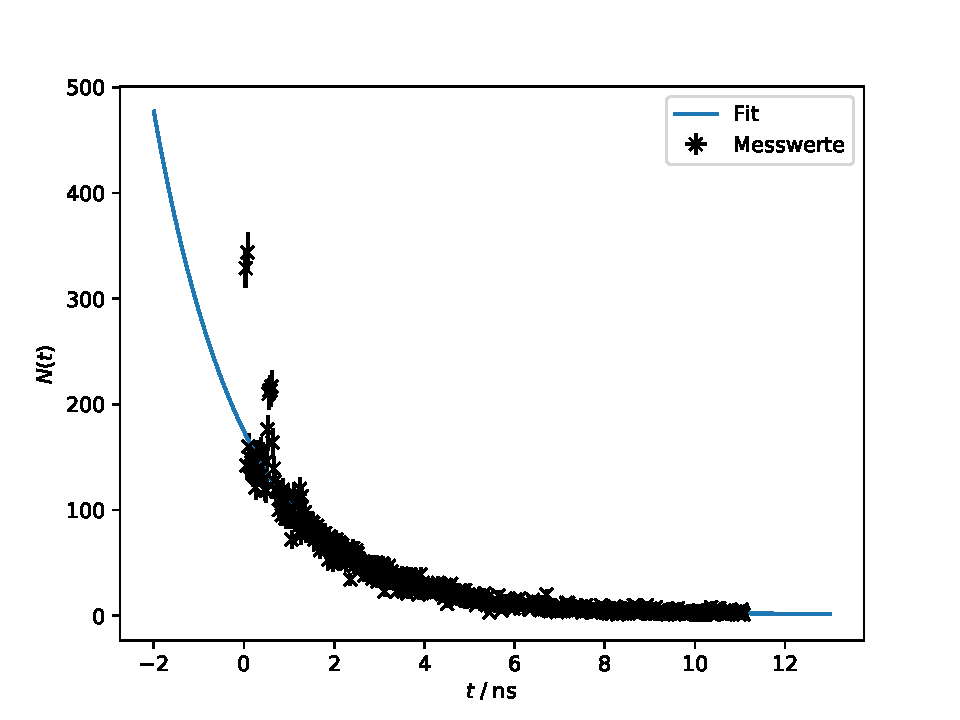
\includegraphics{myonen.pdf}
  \caption{Die Gemessenen Signale über die in Zeitabstände umgewandelten Channels, sowie die Regression.}
  \label{fig:myonen}
\end{figure}

\begin{figure}[h]
  \centering
  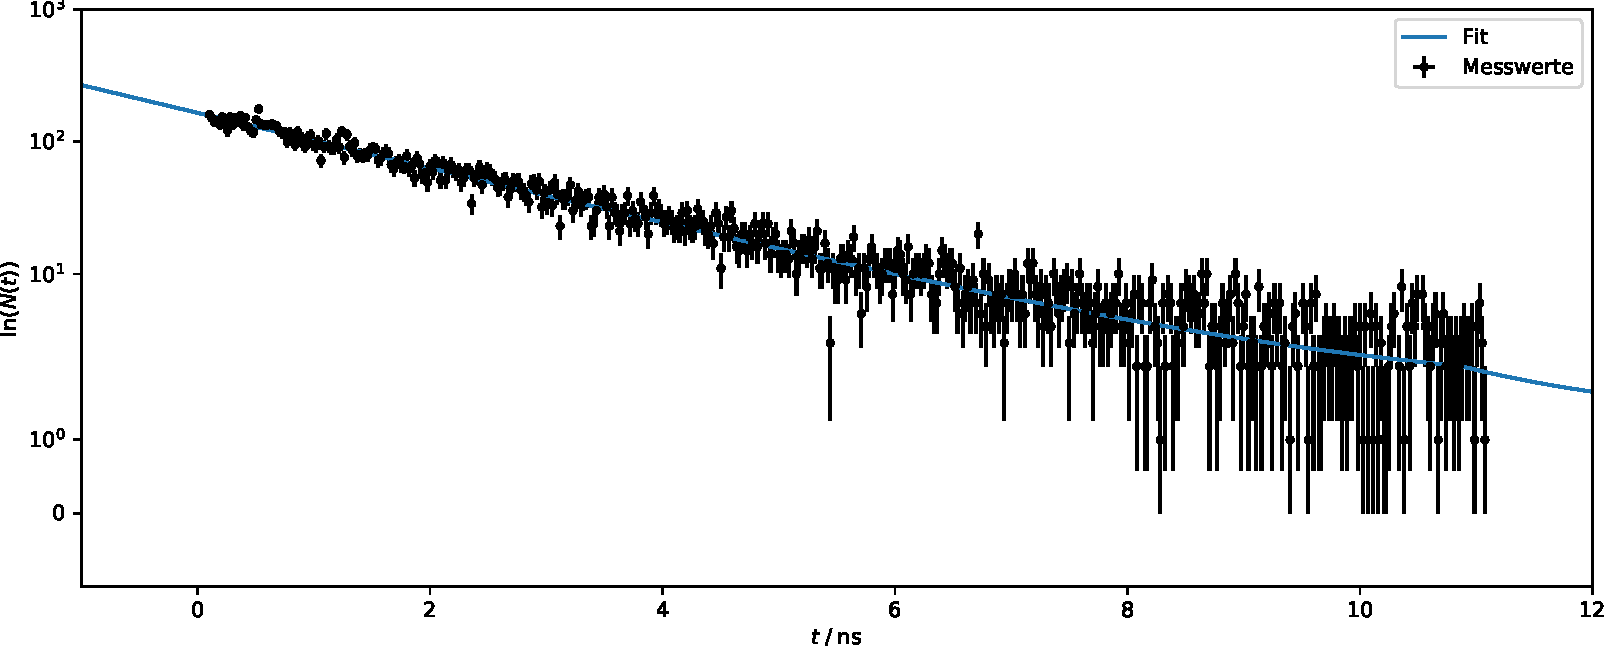
\includegraphics[width=1.2\textwidth]{myonen_log.pdf}
  \caption{Die Gemessenen Signale über die in Zeitabstände umgewandelten Channels, sowie die Regression in logarithmischer Darstellung.}
  \label{fig:myonen_log}
\end{figure}
